\section{Introduction}
C provides different kinds of data types to store the various values e.g. integer, decimal and strings etc. as shown in Listing \ref{c:variableEx}. These data types can be categorized in two ways i.e. `built-in data types' and `user defined data types'; which can be further classified as `variables' and `constants'. In this chapter, these data types are discussed.

\section{Variable example}
Before discussing the data types, let us see one example of variables and their types. In Listing \ref{c:variableEx}, three \textbf{variables} are defined i.e. x and z of integer type (Line 7) and y of float type (Line 8), using `int' and `float' keyword respectively. Note that, the `float' and `int' keywords are used to store `decimal' and `integer' values respectively.



Next, the values of `x' and `y' are set to 2 and 2.7 in Lines 10 and 11 respectively. Finally, these two values are added in Line 12, whose output is 4 (not 4.7). The decimal values is ignore in the output because `z' is declared as `int', which can store only `integer' values, not the `float' values. 
\lstinputlisting[
language = C,
caption    = {Variable and data type},
label      = {c:variableEx}
]{variableEx.c}

\section{Built-in data types}
Table \ref{tbl:dataTypes} presents the 5 built-in data types, which are essential for design purposes. The data types in Table \ref{tbl:dataTypes},  can be further mixed with the other keywords i.e. `signed', `unsigned', `short' and `long', which will specify the range and required memory for the variables. Some of these combination are shown in Table \ref{tbl:combineDatatype} along with the required memory sizes and ranges. Lastly, the memory size can be checked for different data types with keyword `sizeof' as shown in Listing \ref{c:dataTypeEx}

\begin{table}[!h]
	\centering
	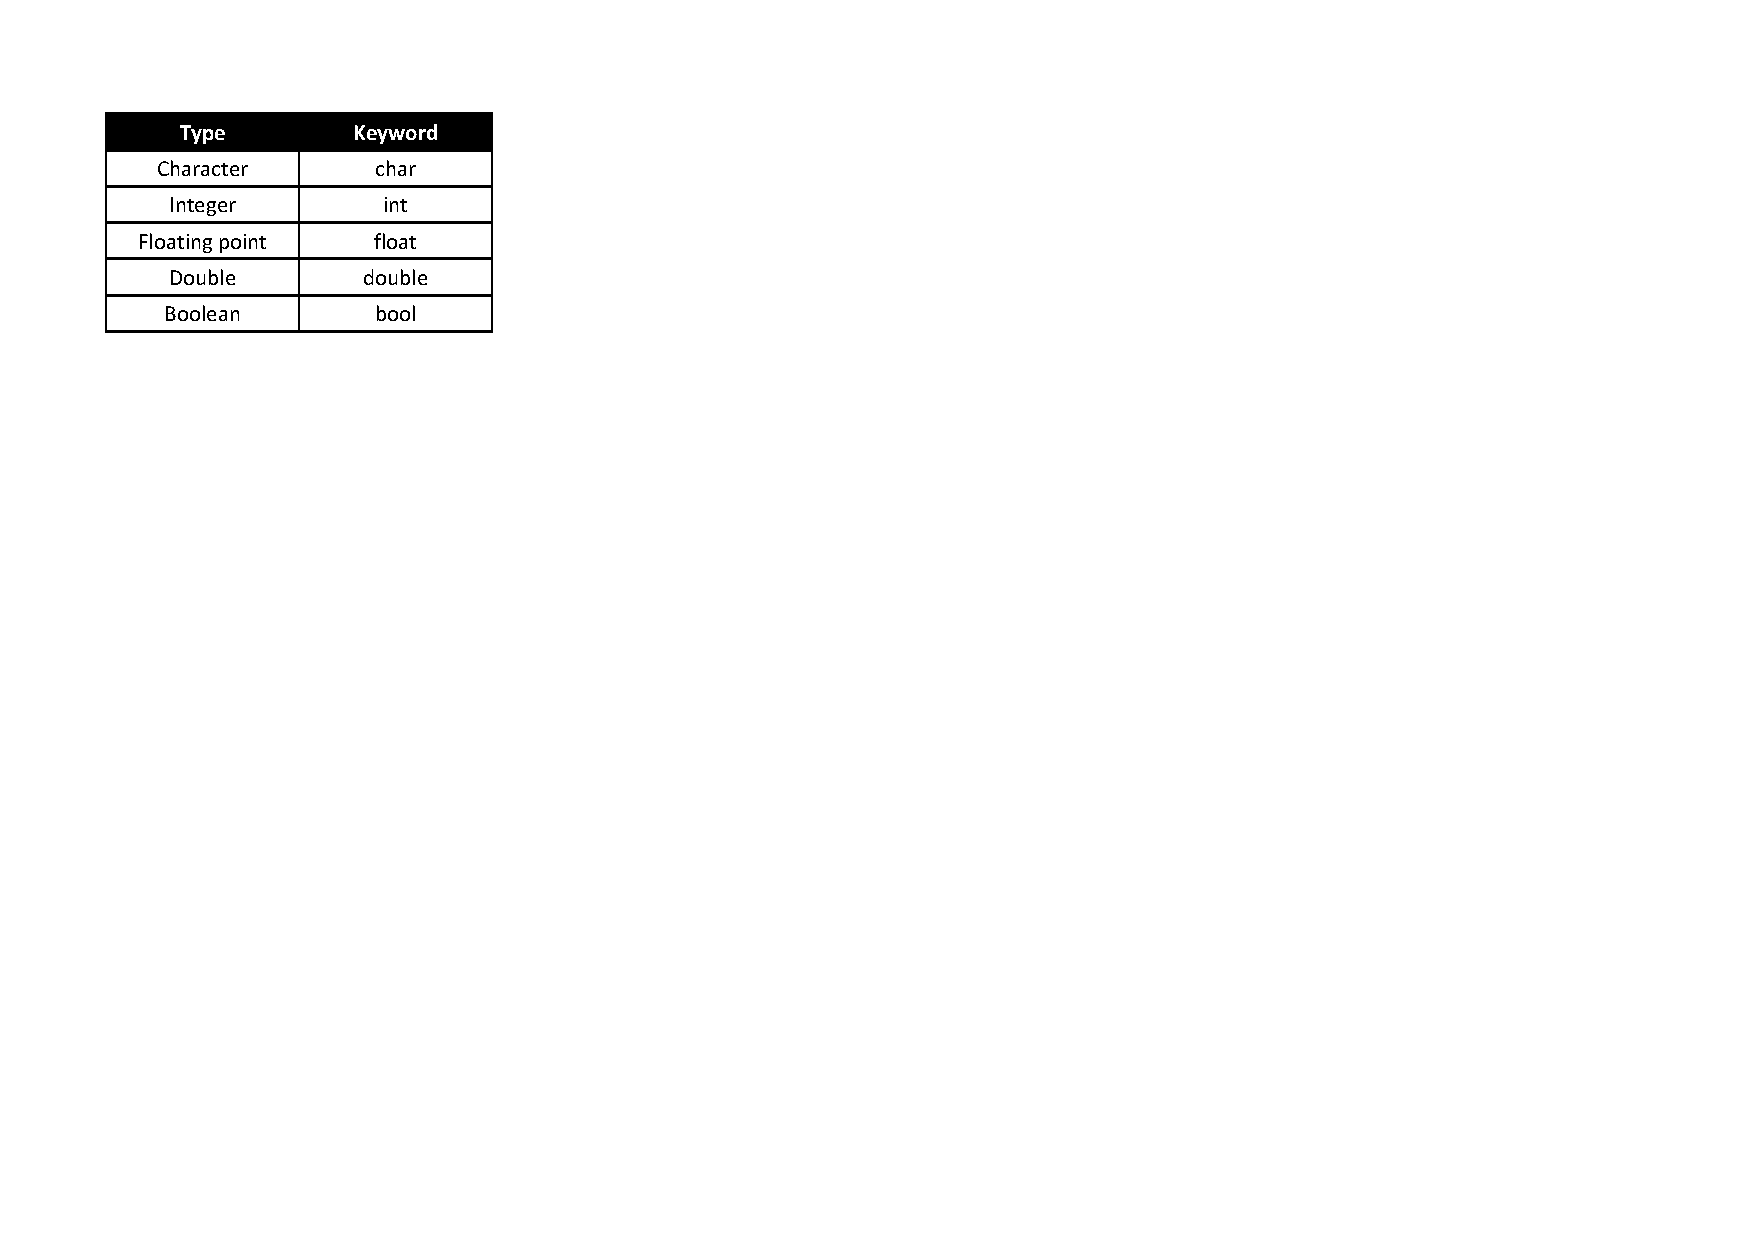
\includegraphics{dataTypes}
	\caption{Built-in data types}
	\label{tbl:dataTypes}
\end{table}

\begin{table}[!h]
	\centering
	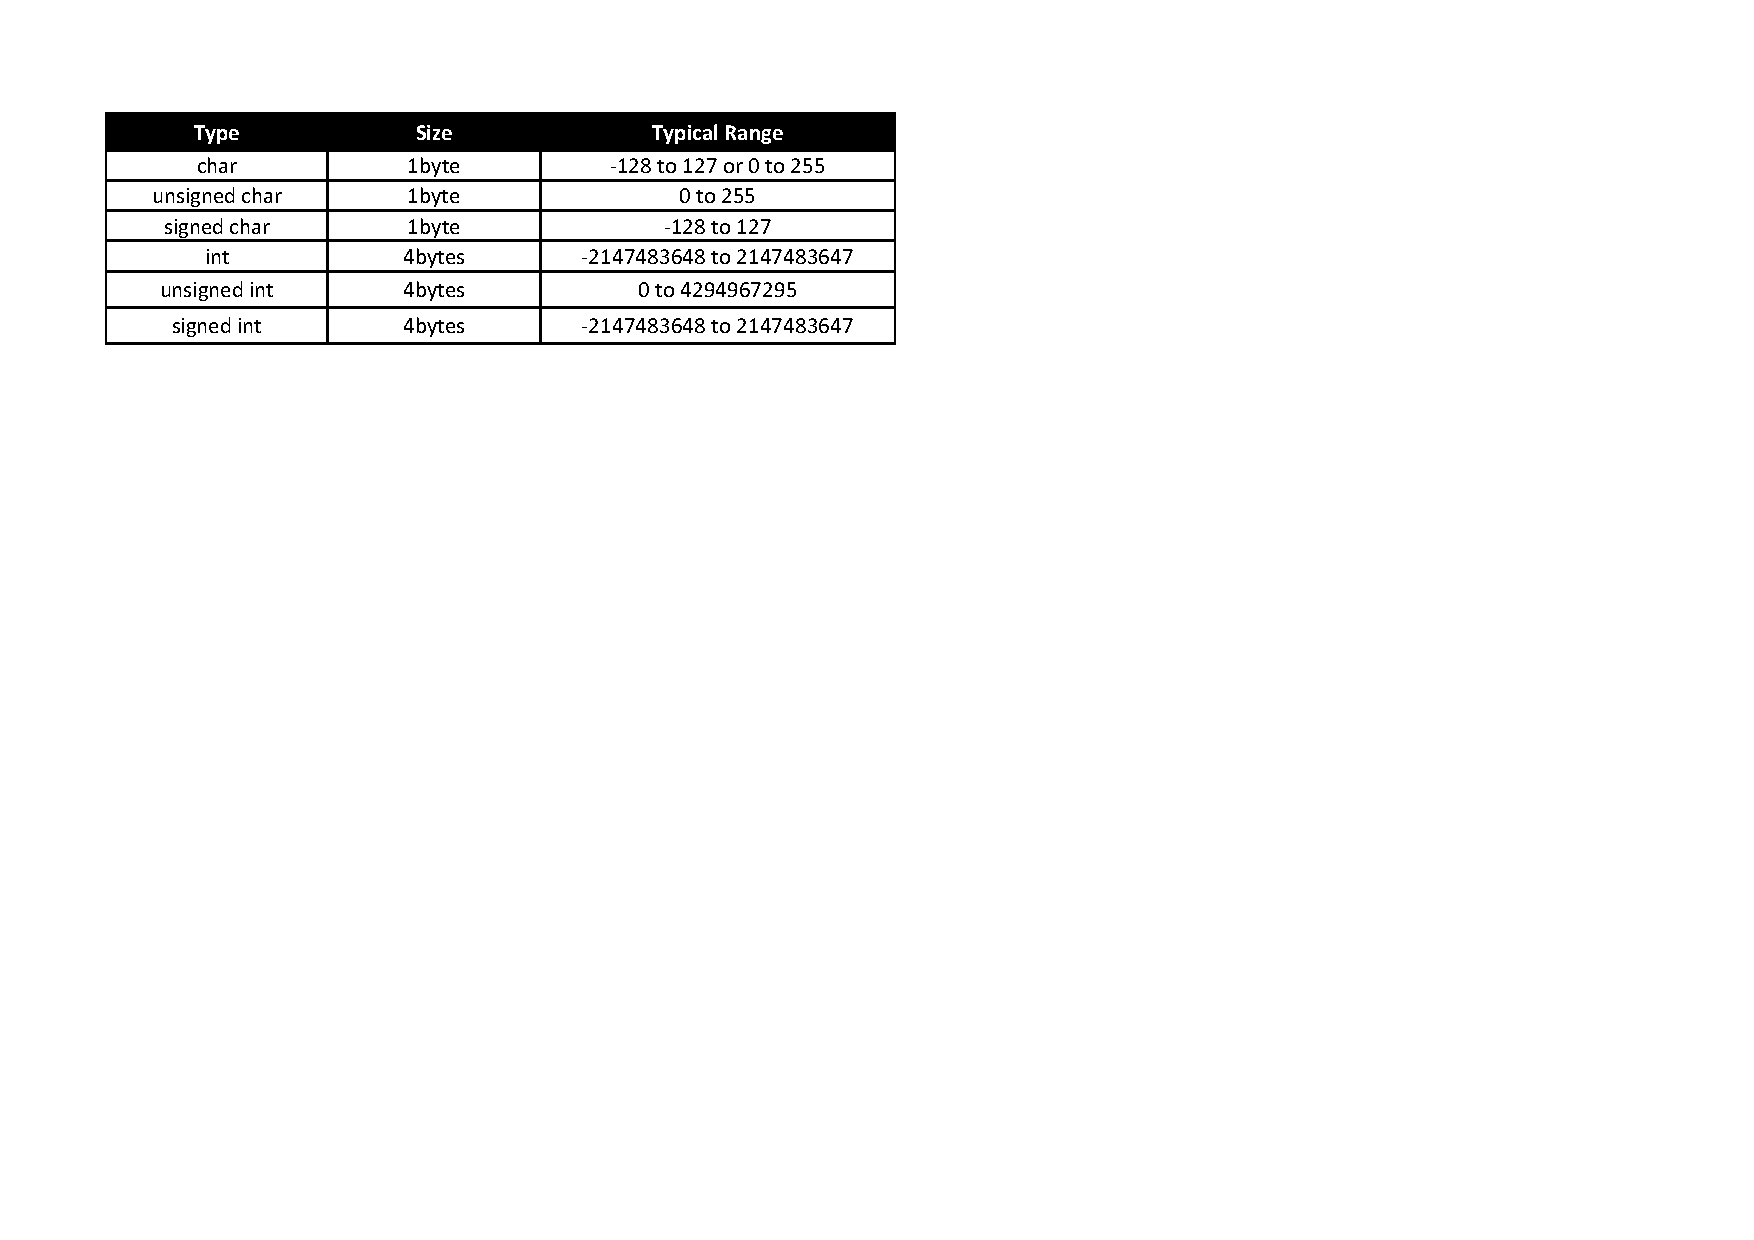
\includegraphics{combineDatatype}
	\caption{Required memory and range for data types}
	\label{tbl:combineDatatype}
\end{table}

\lstinputlisting[
language = C,
caption    = {Required memory for different data types},
label      = {c:dataTypeEx}
]{dataTypeEx.c}

\section{Enumerated data types}
Custom data type can be defined using the keyword `enum', which are known as `enumerated data types'. Listing \ref{c:enumDataEx} presents the example of `enumerated data type'. Note that, `if statement' (at Line 16) is used in this example which is discussed in Section \ref{sec:ifElse}.
\begin{explanation}[Listing \ref{c:enumDataEx}]
	In the listing, `enumerated data type' is defined at Lines 8-10. Here, the data type `stateReg' has two possible values i.e. `Win' and `Loose'. Next, a variable `currentState' of type `stateReg' is defined at Line 12. Then, in Line 13, variable `dice' is declared, with `initial value = 6'. 
	
	In Line 16, `if statement' is used, which is discussed in Section \ref{sec:ifElse}. Lines 16-21 indicates that if dice value is 6, then value of variable `currentState' will be set as `Win', else it will be set as `Loose'. Lastly, Lines 24-27 prints the message based on `currentState' value i.e. if it is `Win' then the message `You won the game' will be printed i.e. Line 25, else Line 27 will be printed. 
	
\end{explanation}
\lstinputlisting[
language = C,
caption    = {Enumerated data type},
label      = {c:enumDataEx}
]{enumDataEx.c}

\section{Constants: define and const}
Constants can be defined in two ways i.e. using `\#define' and `const' keywords as shown in Listing \ref{c:defineConstantEx}.

\begin{explanation}[Listing \ref{c:defineConstantEx}]
	In the listing, one new header is introduced i.e. `math.h'. This header contains various mathematical operations e.g. sin, abs, sqrt and pow etc. In the listing `pow (i.e. power)' is used at Line 14, where area of the circle is calculated i.e. $\pi r^2$. Further, constants are defined using keywords `define' (Line 6) and `const' (Line 11). Then, these two constant values are used at Line 14 to calculate the area. Constant at Line 7 is used to show that a string can be defined as constant as well; which is used at Line 17 with `printf' statement. Also, note that constants can not be modified e.g. if you uncomment the Lines 19 or 20, then error will be generated. 
\end{explanation}
\lstinputlisting[
language = C,
caption    = {Constants: define and const},
label      = {c:defineConstantEx}
]{defineConstantEx.c}


\section{Reading data from terminal with `scanf'}

Listing \ref{c:scanfEx} shows the usage of `scanf' command for getting data from the users. 


\begin{explanation}[Listing \ref{c:scanfEx}]
In the listing, at Line 7, variable `name' is defined of type `char' with maximum length 30 i.e. char[30]. When we run the code, after execution of Line 9, the message `Enter your name' will be displayed. Note that, $\backslash t$ is used in Line 9, which puts the one-tab-space after the message. Next, compiler will stop at Line 10, to get the input value from the user for the variable `name'. Once, we provide the name e.g. Meher, the compiler will go to next line and print the message `Hello Meher'. 

Further, `scanf' command reads the input values from the user till a white space appear, i.e. if we type the value as `Meher Krishna', the compiler will read the word `Meher' only, as there is white space after that and the second part will be omitted from the result.  
\end{explanation}

\begin{noNumBox}
	Lastly, see Listing \ref{c:scanfEx2} for more `scanf' commands; \textbf{also see the comments carefully in the listing}. It's better to put one space before \% sign, in every scanf-statement to avoid problems, as we did in Line 19 of Listing \ref{c:scanfEx2}.
\end{noNumBox}

\lstinputlisting[
language = C,
caption    = {Getting data from user using `scanf'},
label      = {c:scanfEx}
]{scanfEx.c}

\lstinputlisting[
language = C,
caption    = {More `scanf' commands : look comments carefully},
label      = {c:scanfEx2}
]{scanfEx2.c}

\begin{noNumBox}
Note that, the `character (char a)' is initialized within `single quote' whereas the character-array (char a[ ]) is initialized within `double quote' as shown in Lines 9 and 10 respectively of Listing \ref{c:scanfEx2}. 
\end{noNumBox}

\section{Character array}\label{sec:chArray}
In Listing \ref{c:scanfEx2}, we saw that the datatype `char' can store only 1 character; whereas character-array can store multiple character based on it's size. Character array can be defined in two ways e.g. character array `a' can be defined as `\textbf{char a[ ]}' and `\textbf{const char *a}', as shown in Listing \ref{c:charArrayEx}. Note that, `char [a]' value can not be assigned directly in the program (Line 12), but it can be obtained using `scanf' command (Line 14); whereas value can be assigned to `const char *a' in the program (Line 17), but it can not be obtained by using `scanf' command. Please uncomment these lines to see the errors. 

\lstinputlisting[
language = C,
caption    = {Character array},
label      = {c:charArrayEx}
]{charArrayEx.c}

\section{Conclusion}
In this chapter, we saw the basic data types i.e. `in-built data types' and `user-defined data types'. Further, these data types are used as `constant' and `variables'. In next chapter, we will see various operators and control structures to use these data types for performing various tasks. 